\documentclass[a4paper,11pt, twoside]{article}
\usepackage[top=2.5cm,bottom=3cm, inner=3cm, outer=2.5cm]{geometry}
\usepackage[utf8]{inputenc}
\usepackage[activeacute,spanish]{babel}
\usepackage{amsmath,amssymb,amsthm,amscd}
\usepackage{pdfpages}
\usepackage{listings}
\usepackage{setspace}
\usepackage{parskip}
\usepackage{graphicx}
\usepackage[explicit]{titlesec}
\usepackage[font=small]{caption}   
\usepackage{times}
\usepackage{courier}
\usepackage{subfigure}
\usepackage{longtable}
\usepackage[title]{appendix}
\usepackage{afterpage}
\usepackage{fancyhdr}
\usepackage[bookmarks = true, colorlinks=true, linkcolor = black, citecolor = black, menucolor = black, urlcolor = black]{hyperref}
\usepackage{color}
\usepackage{titlesec}
\usepackage{enumitem}
\usepackage{tabularx}

\setlength\parindent{0pt}

\renewcommand{\rmdefault}{phv} % Arial
\renewcommand{\sfdefault}{phv} % Arial

\graphicspath{ {imagenes/} }

\setlength{\parindent}{0.5cm}
\renewcommand*{\thepage}{\footnotesize\arabic{page}}
\renewcommand\spanishfigurename{\textbf{Figura}}
\renewcommand\spanishtablename{\textbf{Tabla}}
\renewcommand\spanishcontentsname{\Large{Índice de contenidos}}
\renewcommand{\appendixname}{Anexos}
\renewcommand{\appendixtocname}{Anexos}
\renewcommand{\appendixpagename}{Anexos}
\newcommand\blankpage{\null\thispagestyle{empty}\addtocounter{page}{-1}\newpage}

\newcolumntype{M}[1]{>{\centering\arraybackslash}m{#1}}
\newcolumntype{C}[1]{>{\centering\arraybackslash}p{#1}} % centered version of 'X' columns


\title{Diseño e implementación de un sistema experto de ayuda a la detección de síndromes basado en puntos característicos de la cara.}

\lstdefinestyle{codeLST}{           
  belowcaptionskip=1\baselineskip,
  breaklines=true,
  frame=tb,
  xleftmargin=\parindent,
  xrightmargin=\parindent,
  language=C,
  showstringspaces=false,
  basicstyle=\footnotesize\ttfamily
}

\pagestyle{fancy}
\fancyhf{}
\renewcommand\headrulewidth{0pt}
\fancyfoot[LO,RE]{\thepage}
\cfoot{}
\titlespacing*{\section}
{0pt}{0ex}{0ex}
\titlespacing*{\subsection}
{0pt}{0ex}{0ex}
\titlespacing*{\subsubsection}
{0pt}{0ex}{0ex}
\pagenumbering{roman}

\begin{document}
\renewcommand{\listtablename}{Índice de tablas}

\afterpage{\blankpage}    
\begin{titlepage}
        \begin{center}
            \vfill
            {\fontfamily{pnc} \fontsize{18}{21.6}\selectfont \textbf{Universidad de Valladolid}}
            \\
            \vspace*{1in}
            \begin{large}
                {\fontsize{26}{31.2}\selectfont E.T.S Ingeniería Informática}
            \end{large}\\
            \vspace*{0.25in}
            {\fontfamily{ptm} \fontsize{13}{15.6}\selectfont \textbf{Prácticas en empresa}}\\
            \vspace*{0.6in}
            {\fontsize{16}{19.2}\selectfont Grado en Ingeniería Informática\\
Mención Ingeniería de Software}\\
            \vspace*{0.8in}
            {\fontsize{28}{33.6}\selectfont \textbf{Diseño e implementación de una aplicación para impresión 3D}}\\
            \vspace*{1.1in}
            \begin{flushright}
                {\fontfamily{cmr}\fontsize{17.28}{20.74}\selectfont Autor:\\
                \textbf{Dña: Andrea Escribano García} \\}
                \vspace*{0.1in}
                {\fontfamily{cmr} \fontsize{17.28}{20.74}\selectfont
                Tutor:\\
                \textbf{Dña. Maria Carmen Hernández Diez }\\}
            \end{flushright}

        \end{center}
    \end{titlepage}
    
\setlength{\parindent}{0.5cm}
\setcounter{page}{1}
\section*{Resumen}

\newpage
\thispagestyle{empty}
\tableofcontents
\cleardoublepage
\thispagestyle{empty}
\listoffigures % indice de figuras

\cleardoublepage
\thispagestyle{empty}
\listoftables % indice de tablas

\newpage
\setcounter{page}{1}
\pagenumbering{arabic}
\section{Introducción}
\subsection{Propósito, alcance y objetivos} 
El propósito de la realización de este programa es la necesidad tecnológica de un cliente. Es decir, necesita de este proyecto para poder manejar un proyecto más grande.

El alcance relacionado con el programa es:
\vspace{-2.5mm}
\begin{itemize}[noitemsep,topsep=0pt]
   \item Escoger una fotorafía de una figura en 3D.
   \item Ser capaz de tratar esa imagen por capas. (Dependiendo del láser.)
   \item Comunicarse con la impresora y enviarle todos los datos calculados.
%   {\color{magenta} \item Visualizar o corregir la imagen elegida.}
\end{itemize}

Los objetivos de esta aplicacion son: importar imágenes en 3D e imprimir la imagen en 3D.
\subsection{Suposiciones y limitaciones}
Debe existir una lista de suposiciones y limitaciones que deberá cumplir nuestro programa:
\vspace{-2.5mm}
\begin{itemize}[noitemsep,topsep=0pt]
\item Deberá utilizar imagenes con formato 3D, a saber: .iges, .stp, .ply, .wrl, .stl, .obj. {\color{magenta}Todos ellos dependiendo del tipo de láser elegido}.
\item Deberá utilizar un láser específico.
\item Podrán ser utilizados varios materiales, {\color{magenta}pero dependiendo del láser elegido}.
\item Deberá tener una temperatura el láser y la base diferentes entre ellas, pero la misma dependiendo de los materiales a usar.
\item Se podrán establecer varios tamaños en el grosor de las capas, {\color{magenta}dependiendo del láser}.
\item Será capaz de mover la imagen, es decir, el ángulo con el que se quiere imprimir la imagen.
{\color{magenta} \item FALTAN MÁS PERO DEPENDE DEL LÁSER}
\end{itemize}
\subsection{Calendario}
A continuación se expondrá un calendario aproximado de las fases que constituyen esta aplicación. Se tendrá en cuenta los posibles cambios que se puedan aplicar a lo largo del proyecto.
\begin{table}[!h]
 \centering
\begin{tabular}{|M{2.65cm}|M{2.65cm}|M{2.65cm}|M{2.65cm}|M{2.65cm}|}
 \hline
 \textbf{\large Fase} & \textbf{\large Fecha de inicio} & \textbf{\large Fecha de fin} & \textbf{\large Duración estimada (horas) } & \textbf{\large Duración real (horas)} \\\hline
    Creación del plan de proyecto & 16/02/2016 & 21/02/2016 & 38 & 30 \\
        \hline
        Documento de análisis de la aplicación & 22/02/2016 & 01/03/2016 & 59 &  \\
        \hline
        Diseño del prototipo & 02/03/2016 & 05/03/2016 & 22 &  \\
        \hline
        Implementación & 07/03/2016 & 16/03/2016 & 58 &  \\
        \hline
        Pruebas & 17/03/2016 & 22/03/2016 & 20 &  \\
        \hline
        \textbf{\large Total} & {\large}  &{\large} & {\large 197 (300) } & {\large} \\
        \hline
\end{tabular}
        \caption{Calendario.}
		\label{ta:cal}
\end{table}

Se ha desarrollado de lunes a viernes en horario de trabajo de 9:00 a 14:00.

\section{Planificación}
\subsection{Organización del proyecto}
\subsubsection{Roles y responsabilidades}
Al realizar este proyecto en solitario los roles y responsabilidades no son muy relevantes, pero son importantes en el hecho de qué rol tomaremos en cada fase del proyecto.
\begin{itemize}[noitemsep,topsep=0pt]
\item \textbf{Jefe de proyecto}: es aquella persona responsable en alcanzar los objetivos del proyecto para ello tiene que: 
\begin{enumerate}
\item Identificar los requisitos.
\item Establecer unos objetivos claros y posibles de realizar.
\item Equilibrar las demandas concurrentes de calidad, alcance, tiempo y coste.
\item Adaptar las especificaciones, los planes y el enfoque a las diversas inquietudes y expectativas de los diferentes interesados.
\end{enumerate}
Con esto se asegura de realizar todas las actividades planificadas, de terminarlas a tiempo, de que sean de calidad, que cumplan la especificación y queden dentro del presupuesto.
\bigskip
\item \textbf{Analista}: es el encargado de producir una especificación para un sistema que satisfaga las necesidad de nuestro cliente. Es el encargado de trabajar estrechamente con el personal de todas las categorías para averiguar los problemas que surjan en el sistema existente, y cumplir las expectativas.
\bigskip
\item \textbf{Diseñador}: es la persona o grupo de personas que se encargan de definir la arquitectura del sistema, los componentes, los módulos y los datos de la aplicación para que cumplan los requisitos. Utilizan una combinación de habilidades gráficas y de las tecnologías de información para crear el diseño.
\bigskip
\item \textbf{Programador}: es el encargado de escribir, depurar y mantener el código fuente de nuestra aplicación, es decir, escriben las instrucciones en un lenguaje informático que el ordenador puede leer y llevar a cabo para realizar tareas.
\bigskip
\item \textbf{Probador}: planifica y lleva a cabo las pruebas de software del programa para comprobar si funciona correctamente. Identifica el riesgo de sufrir errores, detectarlos y comunicarlos. Evalúa el funcionamiento general del software y sugieren formas de mejorarlo.
\end{itemize}

\begin{table}[!h]
\hspace*{1cm}
\centering
\begin{tabular}{|M{7cm}|M{6.5cm}|}
 \hline
 Fase & Andrea Escribano \\
 \hline
 Creación del plan de proyecto & Analista y Jefe de proyecto  \\
 \hline
 Documento de análisis de la aplicación & Analista y Jefe de proyecto \\
 \hline
 Diseño del prototipo & Diseñador y Jefe de proyecto \\
 \hline
 Implementación & Programador y Jefe de proyecto \\
 \hline
 Pruebas &  Probador y Jefe de proyecto\\
 \hline
\end{tabular}
\caption{Asignación de roles según la fase.}
\label{ta:roles}
\end{table}
\subsection{Planes de proceso de gestión}
\subsubsection{Plan de trabajo}
En esta sección se considerarán las actividades, la calendarización de las mismas y los recursos necesarios.
{\color{red} AÑADIR LAS IMÁGENES DE MPP }
\subsubsection{Recursos}
Para realizar y cumplir con todas las actividades son necesarios una serie de recursos que nos ayudarán a llevarlos a cabo. Les hemos dividido en características según el tipo de recurso que sea y hemos realizado una serie de fichas para cada uno que nos expondrán con mayor detalle éstos.

\begin{itemize}
\item \textbf{Trabajo}:

\quad Los recursos de Trabajo son los relacionados con los miembros del equipo de desarrollo, así como miembros del equipo de garantía de calidad y otros semejantes. Cualquier miembro de la organización del cliente que pueda ser necesitado para comprender o participar en actividades específicas.

\bigskip

\begin{table}[!h]
\centering
\begin{tabular}{|M{6cm}|M{8.38cm}|}
\hline
\multicolumn{2}{|c|}{\textbf{Recurso}} \\ \hline
    \textbf{Nombre} & Miembros del equipo. \\
    \hline
        \textbf{Descripción del recurso} & Miembro de organización y realización de la aplicación. \\
        \hline
        \textbf{Informe sobre su disponibilidad} & Durante toda la duración de la creación y ejecución del proyecto \\
        \hline
        \textbf{Fecha de comienzo en la que se precisa el recurso} & 16/02/2016 \\
        \hline
        \textbf{Tiempo durante el cual se precisa el recurso} & Duración completa del proyecto. \\
        \hline
        \textbf{Habilidades técnicas} & \begin{itemize}
        \item Conocer los requisitos.
        \item Manejarse con las herramientas que se precisen.
        \item Conocer la aplicación.
        \end{itemize} \\
        \hline
\end{tabular}
\caption{Recursos: Miembros del equipo.}
\label{ta:MiembEq}
\end{table}

\newpage

\begin{table}[!h]
\centering
\begin{tabular}{|M{6cm}|M{8.38cm}|}
\hline
\multicolumn{2}{|c|}{\textbf{Recurso}} \\ \hline
    \textbf{Nombre} & Miembro de la organización cliente. \\
    \hline
        \textbf{Descripción del recurso} & Cliente o miembro de la organización cliente que sea necesitado para comprender o participar en actividades específicas. \\
        \hline
        \textbf{Informe sobre su disponibilidad} & En todo el periodo de duración de la creación y ejecución del proyecto \\
        \hline
        \textbf{Fecha de comienzo en la que se precisa el recurso} & 16/02/2016 \\
        \hline
        \textbf{Tiempo durante el cual se precisa el recurso} & Duración completa del proyecto. \\
        \hline
        \textbf{Habilidades técnicas} & Conocer los requisitos. \\
        \hline
\end{tabular}
\caption{Recursos: Miembros de la organización cliente.}
\label{ta:MiembOc}
\end{table}

\item \textbf{Equipamiento}:

\quad Los recursos de equipamiento son aquellos relacionados con el material informático así como toda la infraestructura física para su funcionamiento, además de sillas, mesas, etc.

\bigskip

\begin{table}[!h]
\centering
\begin{tabular}{|M{6cm}|M{8.38cm}|}
\hline
\multicolumn{2}{|c|}{\textbf{Recurso}} \\ \hline
    \textbf{Nombre} & Ordenadores. \\
    \hline
        \textbf{Descripción del recurso} & Ordenadores personales con todo el hardware que se necesite.\\
        \hline
        \textbf{Informe sobre su disponibilidad} & Todo el proyecto. \\
        \hline
        \textbf{Fecha de comienzo en la que se precisa el recurso} & 16/02/2016 \\
        \hline
        \textbf{Tiempo durante el cual se precisa el recurso} & Duración completa del proyecto. \\
        \hline
\end{tabular}
\caption{Recursos: Ordenadores.}
\label{ta:Ord}
\end{table}

\item \textbf{Tiempo}:

\bigskip

\begin{table}[!h]
\centering
\begin{tabular}{|M{6cm}|M{8.38cm}|}
\hline
\multicolumn{2}{|c|}{\textbf{Recurso}} \\ \hline
    \textbf{Nombre} & Tiempo. \\
    \hline
        \textbf{Descripción del recurso} & Tiempo necesario para realizar todas las fases y realizar cada Hito. \\
        \hline
        \textbf{Informe sobre su disponibilidad} & Dependiente de los miembros de la organización que realiza la aplicación. \\
        \hline
        \textbf{Fecha de comienzo en la que se precisa el recurso} & 16/02/2016 \\
        \hline
        \textbf{Tiempo durante el cual se precisa el recurso} & Duración completa del proyecto. \\
        \hline
\end{tabular}
\caption{Recursos: Tiempo.}
\label{ta:Tiempo}
\end{table}

\newpage

\item \textbf{Materiales}:

\quad Son aquellos en los que intervienen consumibles de informática, papel, bolígrafos, etc.

\bigskip

\begin{table}[!h]
\centering
\begin{tabular}{|M{6cm}|M{8.38cm}|}
\hline
\multicolumn{2}{|c|}{\textbf{Recurso}} \\ \hline
    \textbf{Nombre} & Papel y lápiz/bolígrafo. \\
    \hline
        \textbf{Descripción del recurso} & Papel necesario para tomar notas o realizar diagramas. \\
        \hline
        \textbf{Informe sobre su disponibilidad} & Todo el proyecto. \\
        \hline
        \textbf{Fecha de comienzo en la que se precisa el recurso} & 16/02/2016 \\
        \hline
        \textbf{Tiempo durante el cual se precisa el recurso} & Duración completa del proyecto. \\
        \hline
\end{tabular}
\caption{Recursos: Papel y lápiz/bolígrafo.}
\label{ta:Pap}
\end{table}

\item \textbf{Espacio}:

\quad Si se está en una organización existente el espacio ya está disponible, pero si hay que contratar personal adicional hay que contar con ello, son posibles recursos que tener en cuenta para el Espacio.

\bigskip

\begin{table}[!h]
\centering
\begin{tabular}{|M{6cm}|M{8.38cm}|}
\hline
\multicolumn{2}{|c|}{\textbf{Recurso}} \\ \hline
    \textbf{Nombre} & Sala de la empresa. \\
    \hline
        \textbf{Descripción del recurso} & Sala de trabajo de la empresa cliente. \\
        \hline
        \textbf{Informe sobre su disponibilidad} & De Lunes a Viernes (No festivos). \\
        \hline
        \textbf{Fecha de comienzo en la que se precisa el recurso} & 16/02/2016 \\
        \hline
        \textbf{Tiempo durante el cual se precisa el recurso} & Duración completa del proyecto. \\
        \hline
\end{tabular}
\caption{Recursos: Sala de trabajo.}
\label{ta:Sala}
\end{table}

\newpage

\item \textbf{Servicios}:

\quad Los recursos de Servicios: algunos proyectos necesitan la contratación de servicios especiales. Por ejemplo implementar un sistema distribuido de área amplia precisa tener en cuenta el momento de disponer los servicios de telecomunicaciones.

\bigskip

\begin{table}[!h]
\centering
\begin{tabular}{|M{6cm}|M{8.38cm}|}
\hline
\multicolumn{2}{|c|}{\textbf{Recurso}} \\ \hline
    \textbf{Nombre} & Internet. \\
    \hline
        \textbf{Descripción del recurso} & Internet necesario en la búsqueda de información y en la utilización de algunas herramientas. \\
        \hline
        \textbf{Informe sobre su disponibilidad} & Completa. \\
        \hline
        \textbf{Fecha de comienzo en la que se precisa el recurso} & 16/02/2016 \\
        \hline
        \textbf{Tiempo durante el cual se precisa el recurso} & Duración completa del proyecto. \\
        \hline
\end{tabular}
\caption{Recursos: Internet.}
\label{ta:Inte}
\end{table}

\bigskip

\begin{table}[!h]
\centering
\begin{tabular}{|M{6cm}|M{8.38cm}|}
\hline
\multicolumn{2}{|c|}{\textbf{Recurso}} \\ \hline
    \textbf{Nombre} & ShareLatex/TexMaker. \\
    \hline
        \textbf{Descripción del recurso} & Herramienta disponible para realización de los documentos. \\
        \hline
        \textbf{Informe sobre su disponibilidad} & Completa. \\
        \hline
        \textbf{Fecha de comienzo en la que se precisa el recurso} & 16/02/2016 \\
        \hline
        \textbf{Tiempo durante el cual se precisa el recurso} & Duración completa del proyecto. \\
        \hline
\end{tabular}
\caption{Recursos: Latex.}
\label{ta:Latex}
\end{table}

\bigskip

\begin{table}[!h]
\centering
\begin{tabular}{|M{6cm}|M{8.38cm}|}
\hline
\multicolumn{2}{|c|}{\textbf{Recurso}} \\ \hline
    \textbf{Nombre} & Eclipse. \\
    \hline
        \textbf{Descripción del recurso} & Herramienta para realizar la programación de la aplicación. \\
        \hline
        \textbf{Informe sobre su disponibilidad} & Completa. \\
        \hline
        \textbf{Fecha de comienzo en la que se precisa el recurso} & {\color{red}  RELLENAR } \\
        \hline
        \textbf{Tiempo durante el cual se precisa el recurso} & Periodo de implementación. \\
        \hline
\end{tabular}
\caption{Recursos: Eclipse.}
\label{ta:Eclip}
\end{table}

\newpage

\begin{table}[!h]
\centering
\begin{tabular}{|M{6cm}|M{8.38cm}|}
\hline
\multicolumn{2}{|c|}{\textbf{Recurso}} \\ \hline
    \textbf{Nombre} & Microsoft Project. \\
    \hline
        \textbf{Descripción del recurso} & Programa de planificación de proyectos. \\
        \hline
        \textbf{Informe sobre su disponibilidad} & Completa. \\
        \hline
        \textbf{Fecha de comienzo en la que se precisa el recurso} & 16/02/2016 \\
        \hline
        \textbf{Tiempo durante el cual se precisa el recurso} & Duración completa del proyecto. \\
        \hline
\end{tabular}
\caption{Recursos: Project}
\label{ta:MPP}
\end{table}

\bigskip

\begin{table}[!h]
\centering
\begin{tabular}{|M{6cm}|M{8.38cm}|}
\hline
\multicolumn{2}{|c|}{\textbf{Recurso}} \\ \hline
    \textbf{Nombre} & Programas  de impresión 3D. \\
    \hline
        \textbf{Descripción del recurso} & Herramienta de código abierto para poder ver cómo trabajan con la impresión de imágenes en 3D. \\
        \hline
        \textbf{Informe sobre su disponibilidad} & Completa. \\
        \hline
        \textbf{Fecha de comienzo en la que se precisa el recurso} & {\color{red}  RELLENAR } \\
        \hline
        \textbf{Tiempo durante el cual se precisa el recurso} & Periodo de diseño. \\
        \hline
\end{tabular}
\caption{Recursos: Programas.}
\label{ta:prog}
\end{table}

\end{itemize}
{\color{red}  SEGURO QUE FALTAN MÁS RECURSOS PERO TODO ES DEPENDIENTE DEL LÁSER A UTILIZAR. } 

\subsubsection{Plan de control}
En esta sección se establecerán los hitos necesarios para realizar con éxito la realización de la aplicación, en concreto cuándo debe de terminar cada parte que llevaremos a cabo en ella.
\begin{enumerate}
\item \textbf{Control de requisitos}

\quad En el caso de que algunos de los requisitos cambien, se deberá aprobar y en el caso de que sea admitido el cambio, se procederá con la replanificación del proyecto.

\item \textbf{Control del calendario}

\quad Para poder cumplir con todos los hitos y con la planificación, se seguirá el calendario propuesto con las actividades y su duración. Además llevar un seguimiento de la duración estimada para cada actividad y duración real que nos ha tomado realizar cada una.

\item \textbf{Control de recursos}

\quad Para el control de los recursos que necesitamos en la realización de la aplicación realizaré las últimas actualizaciones del recurso que lo necesite y llevar un control que no sobrepase el tiempo prefijado y nos lleve a utilizar más tiempo el recurso de lo necesario.

\end{enumerate}

\newpage

\subsubsection{Plan de gestión de riesgos}

\begin{table}[!h]
\centering
\begin{tabular}{|M{5cm}|M{5cm}|M{5cm}|}
\hline
1 & Fecha: 16/02/2016 & Categoría: Proyecto\\
\hline
Título: Baja de un trabajador & Probabilidad: Baja & Fase: Todas las fases \\
\hline
\multicolumn{3}{|M{15cm}|}{Consecuencia: Una actividad quedaría sin poder ser realizada.}\\
\hline
\multicolumn{3}{|M{15 cm}|}{ Descripción: Un trabajador del equipo no se encuentra disponible durante un periodo de tiempo para realizar una tarea que le ha sido asignada.}\\
\hline
\multicolumn{3}{|M{15 cm}|}{ Contexto: Este riesgo puede darse a lo largo de todo el proyecto, en cualquiera de las fases.}\\
\hline
\multicolumn{3}{|M{15 cm}|}{ Análisis: Podría provocar el incumplimiento del plazo de entrega.}\\
\hline
Estrategia: Transferencia &\multicolumn{2}{|M{10 cm}|}{Plan de acción: Reorganizar el trabajo del equipo y asignar su trabajo otro periodo de trabajo con menos carga o ampliando horas de trabajo.}\\
\hline
\end{tabular}
\caption{Riesgos: Baja de un trabajador.}
\label{ta:Baja}
\end{table}

\begin{table}[!h]
\centering
\begin{tabular}{|M{5cm}|M{5cm}|M{5cm}|}
\hline
2 & Fecha: 16/02/2016 & Categoría: Proyecto\\
\hline
Título: No disponer de conexión a Internet  & Probabilidad: Media-Alta & Fase: Todas las fases \\
\hline
\multicolumn{3}{|M{15cm}|}{Consecuencia: Un miembro del equipo no pueda trabajar.}\\
\hline
\multicolumn{3}{|M{15 cm}|}{Descripción:Los miembros del equipo no pueden acceder a los medios compartidos con lo que trabajan por la mala o inexistente conexión a Internet.}\\
\hline
\multicolumn{3}{|M{15 cm}|}{Contexto:Este riesgo puede darse a lo largo de todo el proyecto, en cualquiera de las fases.}\\
\hline
\multicolumn{3}{|M{15 cm}|}{Análisis: Provoca que el miembro del equipo no puedan realizar el trabajo asignado para esa sesión.}\\
\hline
Estrategia: Transferencia(de tiempo) &\multicolumn{2}{|M{10 cm}|}{Plan de acción: Realizar horas extra, cuando se disponga de conexión a Internet.}\\
\hline
\end{tabular}
\caption{Riesgos: Falta conexión.}
\label{ta:Conx}
\end{table}

\begin{table}[!h]
\centering
\begin{tabular}{|M{5cm}|M{5cm}|M{5cm}|}
\hline
3 & Fecha: 16/02/2016 & Categoría: Proyecto\\
\hline
Título: Pérdida o mal funcionamiento de un equipo & Probabilidad: Baja & Fase: Todas las fases \\
\hline
\multicolumn{3}{|M{15cm}|}{Consecuencia: Un miembro del equipo no pueden realizar su trabajo.}\\
\hline
\multicolumn{3}{|M{15 cm}|}{Descripción: Un equipo deja de funcionar correctamente o es extraviado/robado.}\\
\hline
\multicolumn{3}{|M{15 cm}|}{Contexto: Este riesgo puede darse a lo largo de todo el proyecto, en cualquiera de las fases.}\\
\hline
\multicolumn{3}{|M{15 cm}|}{Análisis:Provoca que el miembro del equipo no puedan realizar el trabajo asignado para esa sesión.}\\
\hline
Estrategia: Reserva &\multicolumn{2}{|M{10 cm}|}{Plan de acción: Coger un equipo prestado u otro que haya disponible.}\\
\hline
\end{tabular}
\caption{Riesgos: Equipo.}
\label{ta:Eq}
\end{table}

\newpage

\begin{table}[!h]
\centering
\begin{tabular}{|M{5cm}|M{5cm}|M{5cm}|}
\hline
4 & Fecha: 16/02/2016 & Categoría: Producto \\
\hline
Título: Experiencia insuficiente con el software & Probabilidad: Media & Fase: Desarrollo y Pruebas. \\
\hline
\multicolumn{3}{|M{15cm}|}{Consecuencia: Aumenta el tiempo de resolución de una fase.}\\
\hline
\multicolumn{3}{|M{15 cm}|}{Descripción: Un miembro del equipo no tiene el conocimiento suficiente del software con el que se está trabajando.}\\
\hline
\multicolumn{3}{|M{15 cm}|}{Contexto: Principalmente en las fases de desarrollo y pruebas.}\\
\hline
\multicolumn{3}{|M{15 cm}|}{Análisis: Se produce un retraso en el tiempo de finalización de esa actividad debido a que el trabajador desconoce el software.}\\
\hline
Estrategia: Búsqueda &\multicolumn{2}{|M{10 cm}|}{Plan de acción: La persona implicada puede aprender por su cuenta el manejo del software o pedir ayuda a otros miembro del equipo.}\\
\hline
\end{tabular}
\caption{Riesgos: Experiencia.}
\label{ta:Ex}
\end{table}

\begin{table}[!h]
\centering
\begin{tabular}{|M{5cm}|M{5cm}|M{5cm}|}
\hline
5 & Fecha: 16/02/2016 & Categoría: Proyecto\\
\hline
Título: Cambio de un requisito & Probabilidad: Baja &  Fase: Todas las fases \\
\hline
\multicolumn{3}{|M{15cm}|}{Consecuencia: Repetir parte del informe de análisis.}\\
\hline
\multicolumn{3}{|M{15 cm}|}{Descripción: La interfaz externa decide cambiar algún o algunos requisitos del proyecto.}\\
\hline
\multicolumn{3}{|M{15 cm}|}{Contexto: Puede ocurrir en cualquier fase del proyecto.}\\
\hline
\multicolumn{3}{|M{15 cm}|}{Análisis: Replantear el análisis, y dependiendo de la fase las consecuencias varían. En la fase del análisis sólo hace falta sobrescribir el documento del proyecto, pero en la parte de desarrollo puede implicar además de lo anterior modificar el diseño y parte del desarrollo.}\\
\hline
Estrategia:  &\multicolumn{2}{|M{10 cm}|}{Plan de acción: Modificar el informe de análisis y continuar a partir de ahí.}\\
\hline
\end{tabular}
\caption{Riesgos: Requisito.}
\label{ta:Req}
\end{table}

\begin{table}[!h]
\centering
\begin{tabular}{|M{5cm}|M{5cm}|M{5cm}|}
\hline
6 & Fecha: 16/02/2016 & Categoría: Proceso\\
\hline
Título: No cumplir con la entrega de un hito & Probabilidad: Media-Alta &  Fase: Todas las fases \\
\hline
\multicolumn{3}{|M{15cm}|}{Consecuencia: Afecta al resto de entregas del resto de hitos.}\\
\hline
\multicolumn{3}{|M{15 cm}|}{Descripción: Cuando llega la fecha de entrega del hito no se han conseguido los objetivos.}\\
\hline
\multicolumn{3}{|M{15 cm}|}{Contexto: Puede no cumplirse un hito de cualquiera de las fases.}\\
\hline
\multicolumn{3}{|M{15 cm}|}{Análisis: Al retrasarse en la entrega del hito actual, el trabajo se retrasa y por lo tanto los hitos siguiente también se retrasan y en consecuencia se retrasa la entrega del proyecto final.}\\
\hline
Estrategia: Transferencia &\multicolumn{2}{|M{10 cm}|}{Plan de acción: Replanificar el siguiente hito para no retrasar el proyecto.}\\
\hline
\end{tabular}
\caption{Riesgos: Entrega de un hito}
\label{ta:Hito}
\end{table}

\newpage

\begin{table}[!h]
\centering
\begin{tabular}{|M{5cm}|M{5cm}|M{5cm}|}
\hline
7 & Fecha: 16/02/2016 & Categoría: Producto\\
\hline
Título: Requisito insuficiente & Probabilidad: Media &  Fase: Análisis \\
\hline
\multicolumn{3}{|M{15cm}|}{Consecuencia: Realización incorrecta del trabajo.}\\
\hline
\multicolumn{3}{|M{15 cm}|}{Descripción: Un requisito no está bien descrito y por lo tanto su interpretación puede ser errónea.}\\
\hline
\multicolumn{3}{|M{15 cm}|}{Contexto: En la fase de análisis del proyecto.}\\
\hline
\multicolumn{3}{|M{15 cm}|}{Análisis: Si la interpretación no es la correcta, no cumplirá las expectativas del cliente.}\\
\hline
Estrategia: Búsqueda &\multicolumn{2}{|M{10 cm}|}{Plan de acción: Hablar con el cliente para comprobar que se entendieron correctamente los requisitos.}\\
\hline
\end{tabular}
\caption{Riesgos: Requisito insuficiente.}
\label{ta:Req1}
\end{table}

\subsection{Planes de procesos técnicos}
\subsubsection{Modelo de proceso}
El modelo de proceso es el que se ha identificado en otros apartados y consistirá en el avance de las fases que constituyen el ciclo de vida.

\begin{itemize}
\item Creación del plan del proyecto: analizar el alcance del proyecto para identificar las actividades, los recursos, el calendario y la duración de las actividades para realizar la planificación del proyecto.
\item Análisis de la aplicación: definir los requisitos y clases con los atributos y funciones que deben de realizar para hacer el funcionamiento que se nos pide.
\item Diseño: realizar los prototipos de la aplicación.
\item Implementación: realizar el código fuente de la aplicación para añadir el funcionamiento pedido.
\item Pruebas: realizar las pruebas necesarias para comprobar que todas las funcionalidades pedidas se realizan correctamente.
\item Despliegue: instalar la aplicación y probarla.
\end{itemize}

Estas fases pueden tener varias iteraciones pero en nuestro caso, sólo vamos a ver una iteración de estas, aunque las que más pueden ser reiterativas son las dos últimas fases ya que si en la fase de pruebas encontramos algún fallo, tenemos que volver a la fase de implementación para solucionarlo. Como podemos ver en el siguiente diagrama:
    \begin{figure}[h]
                \centering
                \subfigure{\includegraphics[scale=0.2, width=0.5\textwidth]{ciclodevida.png}}
                \captionof{figure}{Ciclo de vida.}
            \end{figure}        
            
            \newpage

\subsubsection{Modelos, herramientas y técnicas}
\begin{itemize}[noitemsep,topsep=0pt]
\item Modelos.

\quad Los modelos que se van a utilizar son: los diagramas de clases, los modelos de casos de uso, los modelos de entidad-relación y los modelos de riesgos. 

\item Herramientas.

\quad Para realizar los informes se ha utilizado: "ShareLatex" que es una herramienta online para la realización de los documentos de texto, pero para no depender de la conexión a internet, he utilizado "TexMaker" herramienta para la realización de los documentos de texto y que no requiere internet. Además, para obtener los informes sobre la gestión de nuestro proyecto hemos utilizado "Microsoft Project".

\quad Para la realización de los requisitos y de los casos de uso utilizaremos la herramienta de REM.

\quad En cambio, para la utilización de los diagramas de clases y entidad-relación utilizaremos la herramienta de Astah.

\quad Para la implementación utilizaremos la herramienta de Eclipse donde como lenguaje de programación usaremos Python. Para coordinar y sincronizar el código de todos miembros del equipo se utilizará la web de control de repositorios https://github.com

\item Técnicas.

\quad Las técnicas que voy a utilizar en todos los casos anteriormente descritos son los aprendidos durante la carrera de ingeniería informática, en las diversas asignaturas de análisis y diseño de aplicaciones, como: patrones de diseño, componentes, etc. También utilizamos las plantillas como: las plantillas de recursos, de riesgos y de este propio informe.

\end{itemize}
\subsubsection{Plan de despliegue}
{\color{red} RELLENAR }
\section{Análisis}
A continuación se realiza el análisis del programa.
\subsection{Requisitos}
\ref{ANEXOII}
\subsection{Casos de uso}
  \begin{figure}[h]
                \centering
                \subfigure{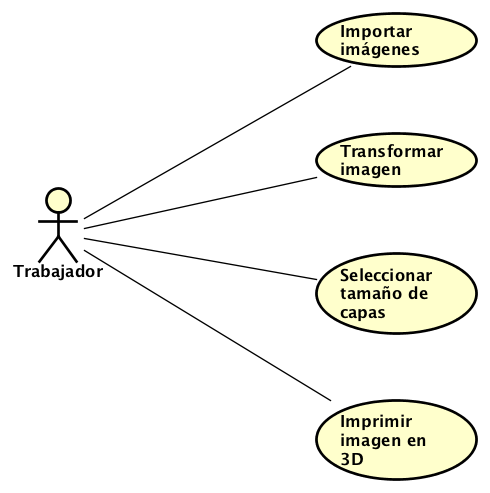
\includegraphics[scale=0.3, width=0.8\textwidth]{ModeloCasosUso.png}}
                \captionof{figure}{Modelo de casos de uso.}
            \end{figure} 
            \newpage
\subsection{Modelo de dominio}
 \begin{figure}[h]
                \centering
                \subfigure{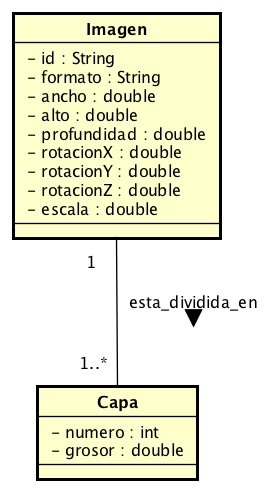
\includegraphics[scale=0.2, width=0.4\textwidth]{ModeloClases.png}}
                \captionof{figure}{Modelo de clases.}
            \end{figure} 
            \newpage
\subsection{Diagrama Entidad-Relación}
\begin{figure}[h]
                \centering
                \subfigure{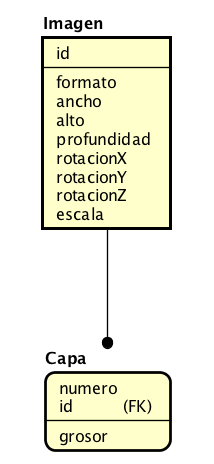
\includegraphics[scale=0.1, width=0.35\textwidth]{ModeloER.png}}
                \captionof{figure}{Modelo Entidad-Relación.}
            \end{figure} 
            
\subsection{Diagrama relacional}
\begin{figure}[h]
                \centering
                \subfigure{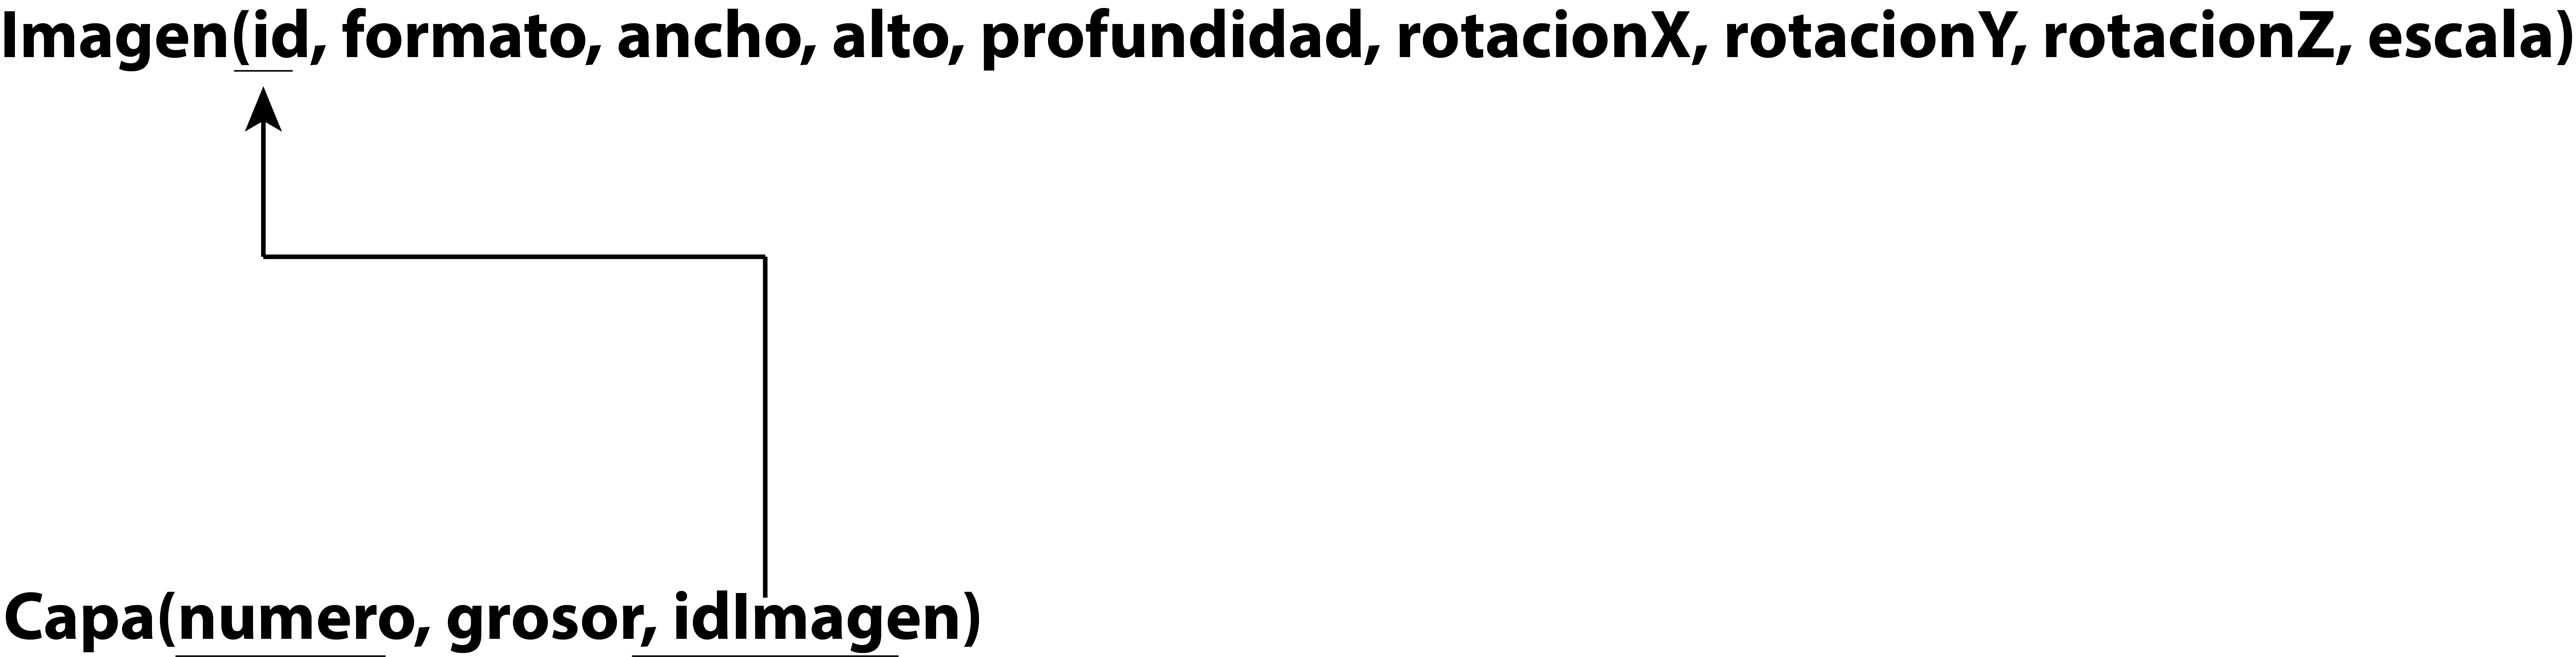
\includegraphics[scale=0.4, width=\textwidth]{ModeloRelacional.png}}
                \captionof{figure}{Modelo Relacional.}
            \end{figure} 
            
\section{Diseño}
\subsection{Aplicaciones similares}
Podemos encontrar varias aplicaciones similares en la impresión de imágenes en 3D.
\vspace{-2.5mm}
\begin{itemize}[noitemsep,topsep=0pt]
\item Slicer: Aplicación de código abierto que ayuda a la impresión 3D y de 2D. No es muy intuitiva pero tiene bastante funcionalidad cuando se trabaja con ella.
\end{itemize}
\section{Implementación}
\section{Pruebas}
\section{Instalación}
\section{Manual de usuario}
\section{Riesgos}
\section{Seguimiento}
\subsection{Plan de seguimiento}
\newpage
\subsubsection{Planificación}
\begin{table}[!h]
\centering
\begin{tabular}{|M{1cm} | M{6cm}| M{3cm} | M{3cm} |}
\hline
\textbf{\large Tarea} & \textbf{\large Nombre} & \textbf{\large Duración Estimada (horas) } & \textbf{\large Duración real (horas) }\\ \hline
1 & Análisis del documento de alcance & 2 & 2 \\ \hline
2 & Realización de una reunión con el cliente & 1 & 1 \\ \hline
3 & Realización del resumen del proyecto & 2 & 1 \\ \hline
4 & Realización de la organización del proyecto & 1 & 1 \\ \hline
5 & Identificación de las actividades & 2 & 1 \\ \hline
6 & Identificación de los recursos & 2 & 1 \\ \hline
7 & Calcular el calendario de las actividades & 2 & 1 \\ \hline
8 & Realización del plan de control & 3 & 1 \\ \hline
9 & Identificación de los riesgos & 2 & 1 \\ \hline
10 & Realización del plan de control de los riesgos & 2 & 2 \\ \hline
11 & Identificación de las herramientas necesarias & 2 & 1 \\ \hline
12 & Realización de planes de los procesos técnicos & 2 & 1 \\ \hline
13 & Revisión del documento & 2 & 1 \\ \hline
14 & Realización de cambios en el documento & 2 & 1 \\ \hline
15 & Realización de documento de seguimiento & 20 & 14 \\ \hline
\end{tabular}
\caption{Seguimiento de la planificación.}
\label{ta:planif}
\end{table}

\newpage

\subsubsection{Análisis}
\begin{table}[!h]
\centering
\begin{tabular}{|M{1cm} | M{6cm}| M{3cm} | M{3cm} |}
\hline
\textbf{\large Tarea} & \textbf{\large Nombre} & \textbf{\large Duración Estimada (horas) } & \textbf{\large Duración real (horas) }\\ \hline
1 & Análisis del documento de la aplicación & 3 & 2 \\ \hline
2 & Identificación de los requisitos funcionales & 3 & 1 \\ \hline
3 & Identificación de los requisitos no funcionales & 2 & 1 \\ \hline
4 & Identificación de los requisitos de información & 1 & 1 \\ \hline
5 & Identificación de las restricciones & 2 & 1 \\ \hline
6 & Identificación de los casos de uso & 2 & 1 \\ \hline
7 & Descripción de los casos de uso & 4 & 2 \\ \hline
8 & Identificación de las clases del modelo del dominio & 5 & 2 \\ \hline
9 & Identificación de las relaciones y multiplicidades & 2 & 2 \\ \hline
10 & Realización del modelo entidad-relación & 3 & 2 \\ \hline
11 & Realización del modelo relacional & 2 & 1 \\ \hline
12 & Revisión del documento & 2 &  \\ \hline
13 &  Realización de cambios en el documento & 3 &  \\ \hline
14 & Realización de documento de seguimiento & 32 &  \\ \hline
\end{tabular}
\caption{Seguimiento del análisis.}
\label{ta:anal}
\end{table}

\subsubsection{Diseño}
\begin{table}[!h]
\centering
\begin{tabular}{|M{1cm} | M{6cm}| M{3cm} | M{3cm} |}
\hline
\textbf{\large Tarea} & \textbf{\large Nombre} & \textbf{\large Duración Estimada (horas) } & \textbf{\large Duración real (horas) }\\ \hline
1 & Investigación sobre los diseños actuales & 3 &  \\ \hline
2 & Realización de los prototipos de las vistas de la aplicación & 3 &  \\ \hline
3 & Revisión de los prototipos & 2 &  \\ \hline
4 & Realización de cambios en el documento & 2 &  \\ \hline
5 & Realización de documento de seguimiento & 12 &  \\ \hline
\end{tabular}
\caption{Seguimiento del diseño.}
\label{ta:dise}
\end{table}

\newpage

\subsubsection{Implementación}
\begin{table}[!h]
\centering
\begin{tabular}{|M{1cm} | M{6cm}| M{3cm} | M{3cm} |}
\hline
\textbf{\large Tarea} & \textbf{\large Nombre} & \textbf{\large Duración Estimada (horas) } & \textbf{\large Duración real (horas) }\\ \hline
1 & Realización y conexión interfaces & 5 &  \\ \hline
2 & Realización de las clases del modelo & 5 &  \\ \hline
3 & Realización de las clases de persitencia & 5 &  \\ \hline
4 & Aplicación de la funcionalidad correspondiente & 6 &  \\ \hline
5 & Realización de las fotos para la obtención de los resultados & 5 &  \\ \hline
6 & Documentación del código & 2 &  \\ \hline
7 & Realización del documento de implementación. & 2 &  \\ \hline
8 & Realización de documento de seguimiento & 28 &  \\ \hline
\end{tabular}
\caption{Seguimiento de la implementación.}
\label{ta:impl}
\end{table}

\subsubsection{Pruebas}
\begin{table}[!h]
\centering
\begin{tabular}{|M{1cm} | M{6cm}| M{3cm} | M{3cm} |}
\hline
\textbf{\large Tarea} & \textbf{\large Nombre} & \textbf{\large Duración Estimada (horas) } & \textbf{\large Duración real (horas) }\\ \hline
1 & Identificación de las diferentes pruebas a realizar & 1 &  \\ \hline
2 & Descripción de las diferentes pruebas a realizar & 2 &  \\ \hline
3 & Ejecución de las pruebas & 2 &  \\ \hline
4 & Realización de cambios en el caso de fallo & 3 &  \\ \hline
5 & Realización del manual de usuario y manual de instrucciones & 2 & \\ \hline
6 &  Realización de documento de seguimiento & 10 &  \\ \hline
\end{tabular}
\caption{Seguimiento de las pruebas.}
\label{ta:prueb}
\end{table}

\subsection{Cambios}
\subsubsection{Generales}
Los cambios más comunes de tiempo han sido por la aparición de otras actividades ajenas a la aplicación y han tenido que variar el inicio o fin de alguna de las actividades planificadas.
\subsubsection{Planificación}
\subsubsection{Análisis}
\subsubsection{Diseño}
\subsubsection{Implementación}
\subsubsection{Pruebas}
\section{Conclusiones.}
\newpage
\renewcommand\refname{Bibliografía}
\begin{thebibliography}{99}
\addcontentsline{toc}{section}{Bibliografía}
    \bibitem{Sciamachy Data Centre}Software Project Management Plan \url{https://aulas.inf.uva.es/pluginfile.php/26264/mod_resource/content/0/materiales_planif/Ejemplo_sdp.pdf}
    \bibitem{IEEE}Software Project  
Management Plan \url{https://aulas.inf.uva.es/pluginfile.php/26254/mod_resource/content/1/Software\%20Project\%20Plan\%20Template\%20-\%20IEEE\%201058-1998\%20-\%20ISO\%2012207.pdf}
\end{thebibliography}

\newpage

\begin{appendices}
\addappheadtotoc
\addtocontents{toc}{\string\renewcommand\string\l@subsection{\string\@dottedtocline{2}{1.5em}{4.5em}}}
\appendixpage

\renewcommand\thesubsection{Anexo \Roman{subsection}}

\subsection{Definiciones y acrónimos}\label{ANEXOI}
\begin{table}[!h]
        \centering
        \begin{tabular}{|c|c|}
        \hline
        \textbf{\large Acrónimo} & \textbf{\large Definición}\\
        \hline
        \end{tabular}
        \caption{Definiciones y acrónimos.}
        \label{ta:defyacr}
    \end{table}
    
    \subsection{Análisis: Resquisitos}\label{ANEXOII}
    
\includepdf[pages=-,pagecommand={},width=1.4\textwidth]{documento.pdf}
\end{appendices}

\end{document}
